\documentclass[withoutpreface]{cumcmthesis}

\begin{document}

\begin{abstractpage}{线性拟合简述}
    本文主要研究线性拟合问题。
    
    首先,我们介绍了什么是\textbf{线性拟合模型}以及拟合的作用与意义。其次,我们基于常用\textbf{误差函数}的定义,详细推导了\textbf{最小二乘法}求参数的原理和结果。在此基础之上,我们简要地引入了评价拟合模型的两个指标:$SSE,R^2$。最后,我们对一组简单的数据进行了一次函数拟合和二次函数拟合,进行对比,以作为全文的示例和总结。

    \keywords{拟合 \quad 线性 \quad 最小二乘法 \quad 拟合优度 \quad SSE}
\end{abstractpage}

\tocpage 
\section{拟合问题简介}

已知若干数据点,在某种曲线族中寻求一条曲线,使得该曲线在某种准则下,与已知数据点最为接近,这样的问题就称为拟合问题。拟合问题得到的曲线不一定经过每一个已知数据点,但距离它们的误差应当足够小。

拟合方法常常用来揭示数据中隐藏的潜在规律,使得人们可以根据这些规律作出对历史数据的总结、对未来数据的预测。

常见的拟合手段,是使用\textbf{关于参数的线性函数}来进行拟合。即使用形如
\begin{equation}
    \varphi(x) = \theta_0 + \theta_1g_1(x) + \theta_2g_2(x)+\cdots+\theta_n g_n(x)
\end{equation}
的函数来进行拟合。

\section{最小二乘法}

\subsection{误差函数}
衡量拟合曲线与已知数据点之间的误差,最容易想到的是直接让二者的函数值作差取绝对值,即
$$cost(\mathbf{\theta}) = \sum\limits_{i=1}^m |\varphi(\theta,x_i)-y_i|$$

但这样构造的函数由于绝对值的存在,很难最小化。在日常应用中,常常使用残差平方和作为误差函数,又叫损失函数。即
\begin{equation}\label{Eq:1}
    cost(\theta) = \sum \limits_{i=1}^m (\varphi(\theta,x_i)-y_i)^2
    = \sum \limits_{i=1}^m[\theta_0 + \theta_1g_1(x_i) +\cdots+\theta_n g_n(x_i)-y_i]^2
\end{equation}

注意到,因为我们已知数据点$(x_i,y_i)$,所以误差函数$cost(\theta)$是关于参数向量$$\theta=\begin{bmatrix}
    \theta_0 \\
    \theta_1 \\ 
    \vdots \\ 
    \theta_n \\
\end{bmatrix}$$的函数。


\subsection{偏导法最小化损失函数}
\cref{Eq:1}两边对$\theta_j$求偏导,并令偏导等于0(其中$g_0(x_i)=1$)
\begin{equation}\label{Eq:2}
    \frac{\partial{cost(\theta)}}{\partial{\theta_j}}=\sum \limits_{i=1}^m 2[\theta_0 + \theta_1g_1(x_i) +\cdots+\theta_n g_n(x_i)-y_i]g_j(x_i)=0
\end{equation}

化简\cref{Eq:2}得,
\begin{equation}\label{Eq:3}
    [\sum \limits_{i=1}^m g_j(x)]\theta_0 + \sum \limits_{i=1}^m [g_1(x_i)g_j(x_i)]\theta _1+\cdots+ \sum \limits_{i=1}^m [g_n(x_i)g_j(x_i)]\theta _n = \sum \limits_{i=1}^m y_ig_j(x_i)
\end{equation}

\cref{Eq:3}是一个非齐次线性方程组,其系数矩阵
\begin{equation}
    A=\begin{bmatrix}\label{Eq:5}
        m & \sum \limits_{i=1}^m g_1(x_i) &\sum \limits_{i=1}^m g_2(x_i) &\cdots& \sum \limits_{i=1}^m g_n(x_i) \\ 
        \sum \limits_{i=1}^m g_1(x) & \sum \limits_{i=1}^m [g_1^2(x_i)] & \sum \limits_{i=1}^m [g_2(x_i)g_1(x_i)] &  \cdots & \sum \limits_{i=1}^m [g_n(x_i)g_1(x_i)]\\ 
        \sum \limits_{i=1}^m g_2(x) & \sum \limits_{i=1}^m [g_1(x_i)g_2(x_i)] & \sum \limits_{i=1}^m [g_2^2(x_i)] &  \cdots & \sum \limits_{i=1}^m [g_n(x_i)g_2(x_i)] \\ 
        \vdots & \vdots &\vdots &\ddots &\vdots \\ 
        \sum \limits_{i=1}^m g_n(x) & \sum \limits_{i=1}^m [g_1(x_i)g_n(x_i)] & \sum \limits_{i=1}^m [g_2(x_i)g_n(x_i)] &  \cdots & \sum \limits_{i=1}^m [g_n^2(x_i)] \\ 
    \end{bmatrix} = R^T R
\end{equation}

其中,$$R=\begin{bmatrix}
    1 & g_1(x_1) & g_2(x_1) & \cdots & g_n(x_1)  \\ 
    1 & g_1(x_2) & g_2(x_2) & \cdots & g_n(x_2)  \\
    \cdots & \cdots &  \vdots \cdots \\ 
    1 & g_1(x_m) & g_2(x_m) & \cdots & g_n(x_m)  \\
\end{bmatrix}$$

其常数向量
\begin{equation}\label{Eq:6}
    b = \begin{bmatrix}
        \sum\limits_{i=1}^{m} y_i \\ 
        \sum\limits_{i=1}^{m} y_i g_1(x_i) \\ 
        \vdots \\ 
        \sum\limits_{i=1}^{m} y_i g_n(x_i)
    \end{bmatrix}=R^T Y
\end{equation}

若$|A|\ne 0$,由克莱姆法则得$\theta_i$有唯一解($A_i$为用$b$替换$A$的第$i$列得到的矩阵,i从0开始计数) :
\begin{equation}\label{Eq:7}
    \theta_i = \frac{|A_i|}{|A|}
\end{equation},即
\begin{equation}
    \theta = (R^TR)^{-1}R^TY
\end{equation}

特别地,令$\varphi(x) = kx+b$,即$g_1(x)=x$,$n=1$
则由\cref{Eq:5}、\cref{Eq:6}、\cref{Eq:7}得
\begin{equation}
    k = \frac{m \sum\limits_{i=1}^{m}x_i y_i - \sum\limits_{i=1}^{m} x_i\sum\limits_{i=1}^{m} y_i}{m \sum\limits_{i=1}^{m} x_i^2- \sum\limits_{i=1}^{m} x_i \sum\limits_{i=1}^{m} x_i}
\end{equation}
\begin{equation}
    b = \frac{\sum\limits_{i=1}^{m}y_i \sum\limits_{i=1}^{m}x_i^2-\sum\limits_{i=1}^{m} x_i \sum\limits_{i=1}^{m}x_i y_i}{m \sum\limits_{i=1}^{m} x_i^2- \sum\limits_{i=1}^{m} x_i \sum\limits_{i=1}^{m} x_i}
\end{equation}

\section{拟合模型的评估}

一般而言,首先要观察数据的分布趋势,选择尽可能简单但又能反映数据整体分布的函数来进行数据拟合。当下面提到的相关评估指标相差不大的时候,应当选择较为简单的模型。

\subsection{SSE}

SSE(the Sum of Squares due to Error),误差平方和,计算的是拟合数据点和原始数据点之间的差值的平方和。
\begin{equation}
    SSE = \sum\limits_{i=1}^{m} (\hat {y_i} - y_i)^2 
\end{equation}

SSE 越接近于0,说明拟合的效果越好

\subsection{\texorpdfstring{$\mathbf{R^2}$}{}}

$R^2$ (Coefficient of determination) ,判断系数/拟合优度,计算的是回归平方和和总体平方和的相近程度。

\begin{equation}
    \mbox{回归平方和 (Sum of Squares of the Regression)}\quad SSR=\sum\limits_{i=1}^{m} (\hat y_i - \bar y_i)^2
\end{equation}
\begin{equation}
    \mbox{总体平方和 (Total Sum of Squares)}\quad SST=\sum\limits_{i=1}^{m} (y_i - \bar y_i)^2
\end{equation}

在线性拟合的前提下,可以证明$SST = SSE  + SSR$

综上,
\begin{equation}
    R^2 = \frac{SSR}{SST}=\frac{1-SSE}{SST} = 1-\frac{SSE}{SST}
\end{equation}

$R^2$越接近于1,说明拟合的效果越好

\section{线性拟合示例}

已知数据点如\cref{Tab:1},请分别使用一次函数和二次函数对其进行拟合。

\begin{table}[H]
    \centering
    \caption{原始数据点}\label{Tab:1}
    \begin{tabular}{|l|c|c|c|c|c|c|c|c|}
        \hline
        x & 0 & 1& 2& 3& 4& 5& 6& 7 \\ 
        \hline
        y & 27 & 26.8 & 26.5 & 26.3 & 26.1 & 25.7 & 25.3 & 24.8 \\
        \hline
    \end{tabular}
\end{table}

用$\varphi_1(x) = kx +b$拟合得到$k=-0.3035,b=27.1250$,$SSE = 0.1082,R^2 = 0.9728$

用$\varphi_2(x)=ax^2+bx+c$拟合得到$a=-0.1410x^2-0.0232x+26.9625,SSE=0.01767,R^2=0.9955$

\begin{figure}[H]
    \centering
    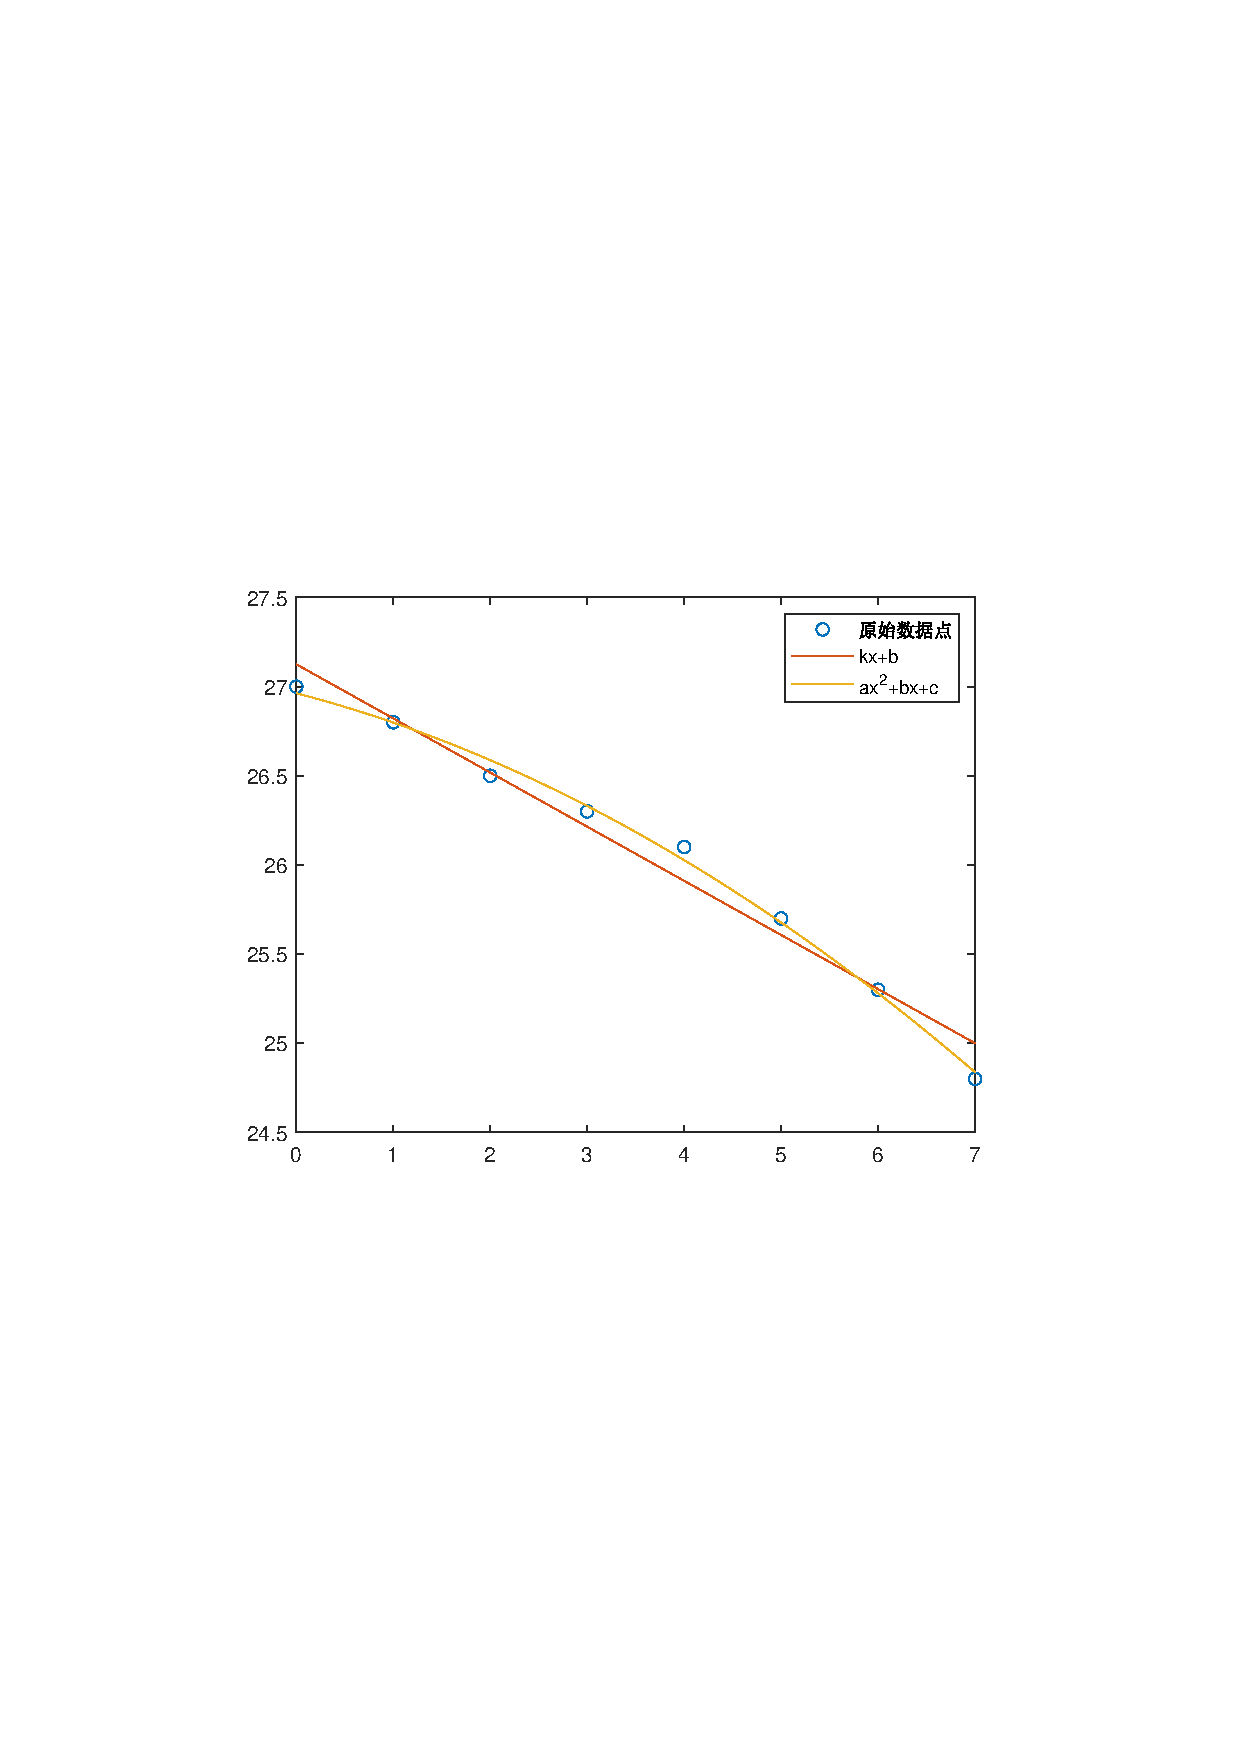
\includegraphics[width=0.8\textwidth]{线性拟合}
    \caption{一次函数与二次函数拟合效果}
\end{figure}

综合各项指标,在没有其他已知条件的前提下,可以认为对已知数据来说,二次函数拟合得更好一些。

\appendix
\section{Matlab 代码}
    \begin{lstlisting}[language=matlab ,caption={自定义的线性拟合函数}]
    function [theta,SSE,R_square] = LinearRegression(x,y,functions)
    % 线性拟合
    % x,y均为列向量
    % functions为元胞函数数组
        
        %% 构造系数矩阵
        m = length(x);
        n = length(functions);
        R = ones(m,n);
        for i = 1:n
            func  = functions{i};
            R(:,i) = func(x);
        end
        
        %% 解正规方程
        A = (R' * R);
        b = R' * y;
        theta =  A \ b;
        
        %% 计算y的拟合值
        hat_y = ones(m,1);
        for i = 1:m
            gi = 0;
            for j = 1:n
            gi = gi+theta(j)*functions{j}(x(i));
            end
            hat_y(i) = gi;
        end
        
        %% 计算SSE和R-square
        mean_y = mean(y);
        SSE = sum((hat_y-y).^2);
        SSR = sum((hat_y-mean_y).^2);
        SST = sum((y-mean_y).^2);
        R_square = SSR/SST;
    end
        
        
    \end{lstlisting}

    \begin{lstlisting}[language=matlab ,caption={一次函数和二次函数拟合比较} ]
    clear,clc

    %% 输入数据
    x = 0:7;
    y = [27;26.8;26.5;26.3;26.1;25.7;25.3;24.8];
    
    %% 输入拟合函数
    f0 = @(x) 1;
    f1 = @(x) x;
    f2 = @(x) x.^2;
    functions1 = {f0,f1};
    functions2 = {f0,f1,f2};
    
    %% kx+b拟合
    [theta1,SSE1,R_square1] = LinearRegression(x',y,functions1);
    
    %% ax^2+bx+c拟合
    [theta2,SSE2,R_square2] = LinearRegression(x',y,functions2);
    
    %% 可视化
    new_x = linspace(min(x),max(x),1000);
    new_y1 = ones(size(new_x));
    new_y2 = ones(size(new_x));
    for i = 1:length(new_x)
        gi1 = 0;
        for j = 1:length(functions1)
            gi1 = gi1+theta1(j)*functions1{j}(new_x(i));
        end
        new_y1(i) = gi1;
        gi2=0;
        for j =1:length(functions2)
            gi2 = gi2+theta2(j)*functions2{j}(new_x(i));
        end
        new_y2(i) = gi2;
    end
    
    plot(x,y,'o',new_x,new_y1,new_x,new_y2)
    legend("原始数据点","kx+b","ax^2+bx+c")
    \end{lstlisting}
\section{Python 代码}

    \begin{lstlisting}[language=python ,caption={初始化} ]
    # 导包
    import numpy as np
    import matplotlib.pyplot as plt
    
    np.set_printoptions(suppress=True)
    
    plt.rcParams["font.sans-serif"] = ["SimHei"]  #设置字体
    plt.rcParams["axes.unicode_minus"] = False  # 解决图像中的“-”负号的乱码问题

    # 初始化数据
    x = np.arange(0, 8)
    y = np.array([27, 26.8, 26.5, 26.3, 26.1, 25.7, 25.3, 24.8])

    # 初始化函数
    f0 = lambda x: 1
    f1 = lambda x: x
    f2 = lambda x: x ** 2
    
    functions1 = [f0,f1]
    functions2 = [f0,f1,f2]
    \end{lstlisting}

    \begin{lstlisting}[language=python ,caption={函数定义} ]
    def LinearRegression(x, y, functions):
    """线性拟合"""
    
        # 参数初始化
        m = len(x)
        n = len(functions)
        R = np.ones((m, n))
    
        for i in range(n):
            func = functions[i]
            R[:, i] = func(x)
    
        # 解正规方程
        A = np.dot(R.T, R)
        b = np.dot(R.T, y)
        theta = np.dot(np.linalg.inv(A), b)
    
        # 计算拟合函数值
        hat_y = np.ones(m)
        for i in range(m):
            gi = 0
            for j in range(n):
                gi = gi + theta[j] * functions[j](x[i])
            hat_y[i] = gi
    
        # 计算SSE和R_square
        mean_y = np.mean(y)
        SSE = np.sum((hat_y - y) ** 2)
        SSR = np.sum((hat_y - mean_y) ** 2)
        SST = np.sum((y - mean_y) ** 2)
        R_square = SSR / SST
    
        return theta, SSE, R_square

    \end{lstlisting}

    \begin{lstlisting}[language=python ,caption={一次函数与二次函数拟合对比} ]
    # kx+b拟合
    theta1,SSE1,R_square1 = LinearRegression(x,y,[f0,f1])
    
    # ax^2+bx+c拟合
    theta2,SSE2,R_square2 = LinearRegression(x,y,[f0,f1,f2])
    
    # 可视化
    new_x = np.linspace(np.min(x),np.max(x),1000)
    new_y1 = np.ones(new_x.shape)
    new_y2 = np.ones(new_x.shape)
    for i in range(len(new_x)):
        gi1 = 0
        for j in range(len(functions1)):
            gi1 = gi1 + np.dot(theta1[j],functions1[j](new_x[i]))
        new_y1[i] = gi1
    
        gi2 = 0
        for j in range(len(functions2)):
            gi2 = gi2 + np.dot(theta2[j],functions2[j](new_x[i]))
        new_y2[i] = gi2
    
    plt.plot(x,y,'o',new_x,new_y1,new_x,new_y2)
    plt.legend(["原始数据点","$kx+b$","$ax^2+bx+c$"])
    \end{lstlisting}
\end{document}